\chapter{20 conceptos más relevantes}

\section{Fundamentos de la Ciberconciencia Situacional}
\begin{enumerate}
\item \textbf{Ciberconciencia Situacional (CS)} \\
La conciencia situacional en el ciberespacio es el concepto fundamental definido como \textit{``la capacidad de saber lo que está sucediendo en el ciberespacio''}. Es esencial porque constituye la base para comprender y reaccionar a las amenazas cibernéticas de manera oportuna y eficaz.
Además, la CS no solo es relevante para la \ul{detección de amenazas}, sino también para la \ul{optimización de recursos de seguridad}, permitiendo priorizar esfuerzos donde realmente se necesitan y evitar la fatiga de alertas que afecta a muchos equipos de seguridad.

\begin{definition}[Situational Awareness]
   Situational awareness is the perception of the elements of the environment within
   a volume of time and space, the comprehension of their meaning, and the
   projection of their status in the near future
\end{definition}

\item \textbf{Ciclo cognitivo de la CS} \\
El ciclo de la CS se compone de adquisición de datos, procesamiento, análisis, distribución y acción. Este ciclo continuo es fundamental porque representa el flujo completo de información desde su captación inicial hasta la toma de decisiones basada en ella, garantizando que la CS \ul{sea un proceso dinámico y no un estado estático}. La efectividad de cada fase impacta directamente en la calidad general de la conciencia situacional, donde fallos en cualquier punto pueden crear puntos ciegos críticos para la seguridad organizacional.

\begin{figure}[htbp]
   \centering
   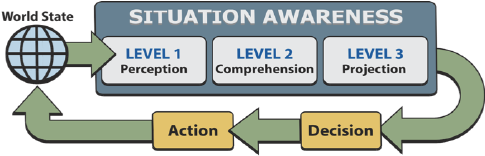
\includegraphics{images/00/cognitive.png}
   \caption{Ciclo cognitivo de la CS}
   \label{fig:00/cognitive}
\end{figure}
\begin{enumerate}
   \item \textbf{Fase de percepción} \\
   Primera etapa del modelo de \textit{Endsley} donde se capturan los datos relevantes del entorno cibernético. Esta fase es crucial porque establece la base informativa sobre la cual se construirá toda interpretación posterior. Una percepción incompleta o distorsionada inevitablemente conducirá a una CS defectuosa independientemente de la sofisticación del análisis posterior. La percepción requiere tanto amplitud como profundidad de visibilidad en el entorno digital para capturar patrones y anomalías significativas.
   
   \item \textbf{Fase de comprensión} \\
   Segunda etapa donde se sintetizan y contextualizan los datos percibidos para crear información significativa. Su importancia radica en transformar datos aislados en un panorama coherente que revela relaciones, patrones y desviaciones significativas. Este proceso integra el conocimiento previo con los datos actuales para determinar la relevancia y el significado de los eventos observados, distinguiendo entre actividades normales y potenciales indicadores de amenaza.
   
   \item \textbf{Fase de proyección} \\
   Tercera etapa que permite anticipar estados futuros basados en la comprensión actual de la situación. Es vital porque transforma la CS de una herramienta puramente descriptiva a una predictiva, permitiendo a las organizaciones pasar de posiciones reactivas a proactivas. La capacidad de proyectar escenarios futuros probables permite anticipar movimientos de atacantes, priorizar vulnerabilidades según la probabilidad de explotación, y asignar recursos defensivos antes de que ocurran los incidentes.
\end{enumerate}
\item[]
\note{Para ver como esto se relacióna a un escenario concreto, podemos hacer algunos ejemplos. La fase de percepción se puede riferir al posicionamiento de sensores y recopilación de datos, la fase de comprensión a la correlación y análisis de datos ---que puede hacer un SIEM---, y la fase de proyección a la predicción de ataques ---a traves de grafos de ataque por ejemplo--- y evaluación de riesgos}
\end{enumerate}


\begin{enumerate}[resume]

\item \textbf{Situation Understanding} \\
El entendimiento situacional va más allá de la simple conciencia situacional, y se refiere a, dada una situació, comprender las posibles consecuencias y predecir eventos futuros. Es relevante porque permite anticipar las amenazas antes de que se materialicen completamente. Mientras que la conciencia situacional responde a la pregunta \textit{``¿qué está pasando?"}, el \textit{entendimiento situacional} busca responder \textit{``¿por qué está pasando y qué podría ocurrir después?"}. Esta profundidad adicional de análisis es fundamental en el complejo entorno cibernético, donde las relaciones causa-efecto no siempre son evidentes y donde un solo indicador puede ser parte de un ataque multifacético más amplio.
\nl

\note{El video de la tarea del sistema idraulico señalaba lo complicado que era distinguir la causa de un problema, porque multiples sensores podrían indicar el mismo problema. En situaciones así, es importante combinar los datos con el conocimiento previo y la experiencia para determinar la causa raíz de un efecto indeseado.}

\item \textbf{Sensemaking} \\
Incluye las actividades cognitivas necesarias para desarrollar conciencia, comprensión y traducirlas en acciones. Es fundamental porque conecta la conciencia con la acción concreta en el dominio cibernético. El proceso de sensemaking representa el puente crítico entre la observación pasiva y la respuesta activa, transformando el conocimiento abstracto en decisiones operativas tangibles. Este proceso involucra la contextualización de la información dentro de marcos mentales preexistentes, la resolución de ambigüedades y contradicciones, y la creación de narrativas coherentes que expliquen los eventos observados.

Para simplificar el proceso de sensemaking es importante disponer de recursos y herramientas apropiados, como sensores, tecnicas de visualización, SIEMs, \dots\\
Pero es importante también destacar que un grafico de visualización de datos no es util sin las inferencias que se pueden hacer tenendo en cuenta el contexto. 
\end{enumerate}

\section{Componentes estructurales de la CS}
\begin{enumerate}[resume]
\item \textbf{Network Awareness} \\
\ul{Componente fundamental que proporciona conocimiento completo sobre los sistemas, redes y activos digitales propios}. Es esencial porque establece la línea base para detectar anomalías y determinar el estado normal de operación.\\
Además, un apropiado particionamento de la red y una segmentación adecuada son una de las primeras líneas de defensa contra las amenazas, y son cruciales para limitar el alcance de un ataque y contener su propagación.

% Sin un conocimiento profundo de la infraestructura propia, las organizaciones no pueden distinguir eficazmente entre comportamientos legítimos y maliciosos, generando exceso de falsos positivos o pasando por alto amenazas reales camufladas como actividades rutinarias.

\item \textbf{Threat Awareness} \\
\ul{Conocimiento sobre las amenazas actuales, emergentes y potenciales que podrían afectar a la organización}. Su importancia radica en proporcionar contexto sobre los actores maliciosos, sus capacidades, motivaciones y tácticas, permitiendo una defensa orientada específicamente a las amenazas más probables y peligrosas para cada entorno particular.\\
Además, conocer las amenazas permite también de mejorar el Situation Understanding, y por tanto también la capacidad de predicir las consecuencias de una determinada situación. 


% Este componente incorpora tanto la inteligencia de amenazas externa como el análisis interno de eventos de seguridad para crear un modelo dinámico del panorama de amenazas relevantes.

\item \textbf{Mission Awareness} \\
\ul{Comprensión de cómo los activos y procesos cibernéticos se relacionan con los objetivos organizacionales críticos}. Es crucial porque alinea las actividades de ciberseguridad con el valor empresarial, permitiendo priorizar la protección de los sistemas y datos que realmente importan para la continuidad y éxito de la misión organizacional. Sin esta perspectiva, las organizaciones pueden desperdiciar recursos protegiendo activos de bajo valor mientras dejan vulnerables componentes críticos para la misión.

% \item \textbf{Niveles de mando CS: Táctico, Operativo y Estratégico} \\
% Esta subdivisión es crucial porque permite adaptar la información a las necesidades específicas de los diferentes niveles decisionales, desde la respuesta técnica inmediata hasta la planificación estratégica. El nivel táctico se enfoca en los detalles técnicos inmediatos necesarios para detectar y responder a incidentes específicos. El nivel operativo coordina múltiples acciones tácticas dentro de un marco temporal más amplio. El nivel estratégico requiere información más abstracta y contextualizada sobre el panorama general de amenazas, riesgos emergentes y su posible impacto en los objetivos organizacionales a largo plazo.
\end{enumerate}

\section{Colaboración y visualización en CS}
\begin{enumerate}[resume]
\item \textbf{Common Operational Picture (COP)} \\
\coolquote{
   A single identical display of relevant (operational) information (e.g. position of own troops and enemy troops, position and status of important infrastructure such as bridges, roads, etc.) shared by more than one Command.
}{\href{https://en.wikipedia.org/wiki/Common_operational_picture}{wikipedia}}
Es fundamental porque proporciona una base común para la conciencia situacional a todos los niveles de mando. 
La COP trasciende la mera representación visual para convertirse en un marco referencial compartido que asegura que todos los actores involucrados en la ciberseguridad interpreten la situación desde una misma perspectiva informativa.\\
La COP se aplica tipicamente en el contexto militar, pero su concepto se ha extendido a la ciberseguridad, donde la necesidad de una visión unificada y coherente de la situación es igualmente crítica.


% \item \textbf{Shared Situational Awareness} \\
% Compartir la misma conciencia entre los miembros del equipo es crucial para garantizar una respuesta coordinada y coherente a las amenazas cibernéticas. Va más allá del COP para incluir no solo la representación visual compartida, sino también un entendimiento común de los objetivos, prioridades, roles y responsabilidades dentro del equipo de respuesta. Esta conciencia compartida actúa como multiplicador de fuerza, permitiendo que equipos distribuidos operen como una entidad cohesionada.

\item \textbf{Visualización de ciberinteligencia} \\
Las técnicas de visualización son fundamentales para representar eficazmente el ciberespacio, compuesto por grandes cantidades de datos complejos y multidimensionales, ayudando a analistas y decisores a identificar rápidamente patrones y anomalías. En el contexto de la ciberdefensa, donde los conjuntos de datos pueden incluir millones de eventos por segundo, las representaciones visuales adecuadas transforman masas amorfas de datos en estructuras comprensibles.
Hemos visto \ul{muchas técnicas de visualización, que no son equivalentes}, y \ul{es importante también elegir la más adecuada para cada contexto}, de lo contrario, los datos podrían seguir siendo incomprensibles o de poca utilidad.
% que aprovechan la capacidad innata del cerebro humano para el reconocimiento de patrones visuales.

\begin{figure}[htbp]
   \centering
   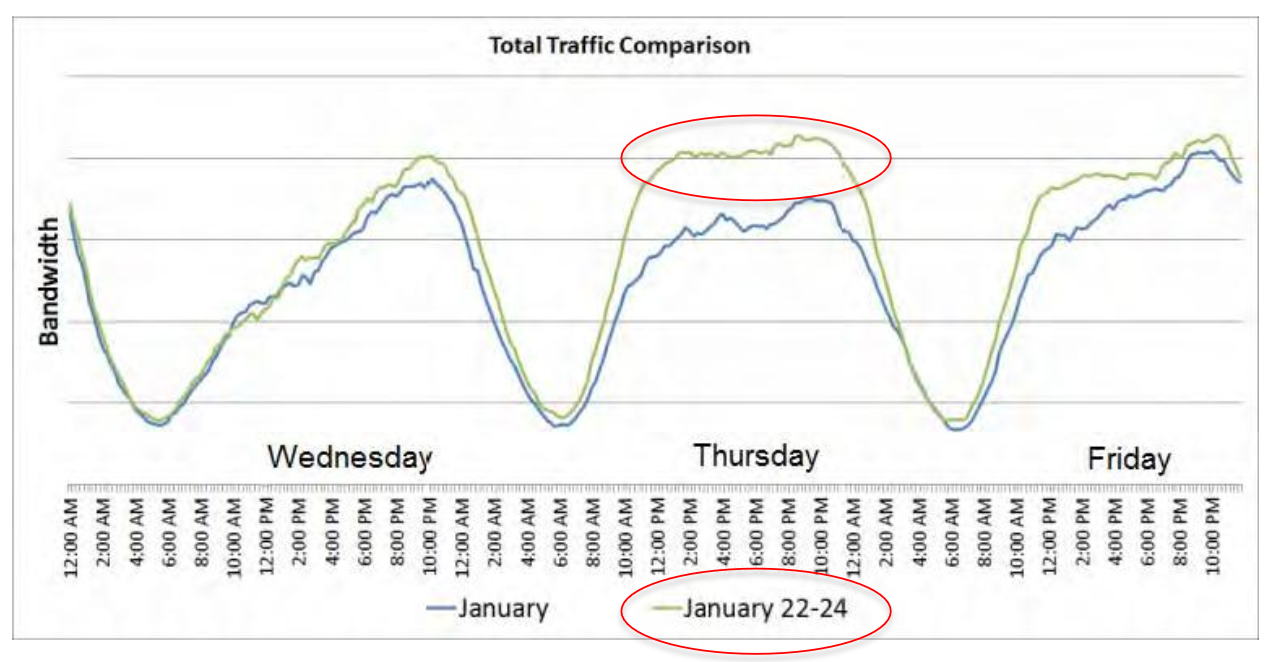
\includegraphics[width=0.49\columnwidth]{images/00/ddos.png}
   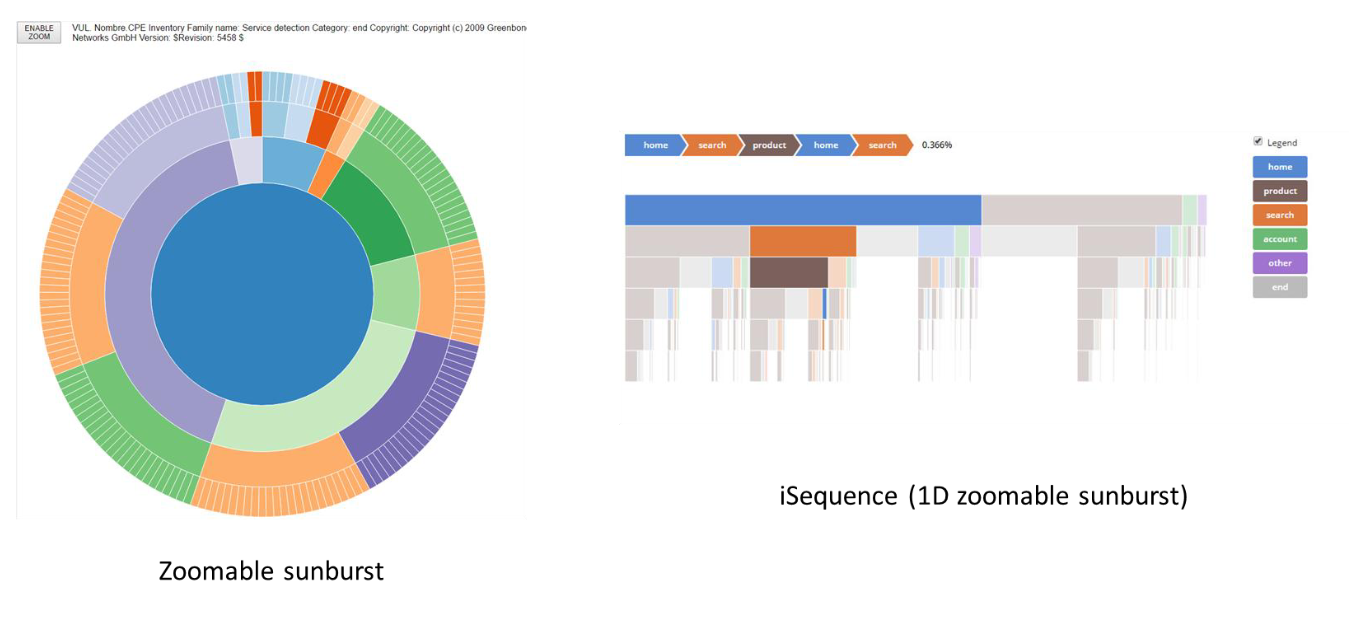
\includegraphics[width=0.49\columnwidth]{images/00/sunburst.png}
   \caption{Ejemplos de visualización de datos}
   \label{fig:00/visualizacion}
\end{figure}

\item \textbf{Gestión de la sobrecarga informativa} \\
Esto se refiere a la importancia de estrategias y técnicas para filtrar, priorizar y presentar \ul{solo la información relevante para cada contexto y rol}.\\

% Es vital porque la cantidad de datos generados en entornos cibernéticos modernos supera ampliamente la capacidad humana de procesamiento, pudiendo conducir a la parálisis analítica o a pasar por alto señales críticas entre el ruido.
Los sistemas efectivos de CS implementan mecanismos de filtrado contextual, agregación inteligente y destacado adaptativo de anomalías para garantizar que cada nivel decisional reciba exactamente la información necesaria en el momento oportuno.
Claro que esto incluye también técnicas de visualización, pero no se limita a eso.
La \textit{Mission Awareness}, puede ayudar a determinar qué información es relevante para cada contexto y, por tanto, también a filtrar la información con mayor eficacia.  
\end{enumerate}

\section{Análisis y gestión de riesgos}
\begin{enumerate}[resume]
% \item \textbf{Análisis de riesgo dinámico} \\
% A diferencia del análisis estático tradicional, este enfoque actualiza continuamente la evaluación del riesgo con datos en tiempo real, esencial en un entorno cibernético en rápida evolución. Los métodos estáticos que evalúan el riesgo en intervalos predefinidos (mensual, trimestral o anualmente) resultan obsoletos en el ciberespacio donde nuevas vulnerabilidades críticas pueden aparecer y ser explotadas en cuestión de horas. El análisis dinámico incorpora constantemente nuevos datos sobre vulnerabilidades emergentes, cambios en la infraestructura, variaciones en las técnicas de ataque y evolución del panorama de amenazas.

\item \textbf{Factores de riesgo} \\
\ul{Amenazas, vulnerabilidades, impacto, probabilidad}, y \ul{condiciónes predisponentes} son elementos clave para cuantificar y priorizar los riesgos en el ciberespacio. 
Estos cinco componentes interrelacionados forman el marco fundamental para una evaluación del riesgo cibernético, permitiendo transformar conceptos abstractos en métricas comparables y accionables. \\
Cada uno de estos se puede descomponer en subcomponentes más específicos, proporcionando un nivel de detalle que permite una evaluación más precisa y granular de los riesgos. Por ejemplo, las amenazas pueden dividirse en fuentes de amenaza y eventos de amenaza, mientras que las vulnerabilidades pueden clasificarse según su naturaleza (técnica, humana, organizativa) o su ubicación (sistemas, procesos, infraestructura).
% El análisis de amenazas identifica actores, motivaciones, capacidades e intenciones de potenciales atacantes. La evaluación de vulnerabilidades examina las debilidades inherentes o introducidas en sistemas. El análisis de impacto cuantifica las consecuencias potenciales, y la evaluación de probabilidad determina la verosimilitud de los incidentes.
\nl

El riesgo es una función de la probabilidad de que se produzca una amenaza y del impacto potencial que sufrirá un activo si se produce el suceso.
El riesgo suele representarse como un valor único, normalmente decimal, o como un vector en el que se evalúan aisladamente distintos tipos de impactos.
\[
risk(e) = probability(e) \times impact(e)
\]
El impacto también puede medirse utilizando la degradación, es decir, el porcentaje \% del activo afectado que se pierde
\[
   impact(e) = value(asset) \times degradation(asset)
\]


\item \textbf{Análisis de consecuencias} \\
Las técnicas para \textbf{evaluar el impacto de los ataques} cibernéticos son cruciales para comprender las potenciales repercusiones operativas y estratégicas de las amenazas.\\
El impacto es un componente crítico del riesgo, y sin su evaluación es dificil evaluar este último.\\
Por ejemplo, hemos mencionado grafos de ataque que representan las relaciones entre vulnerabilidades y cómo los ataques pueden propagarse a través de múltiples sistemas. Estos gráficos permiten visualizar la complejidad de los ataques y sus posibles consecuencias en cascada, facilitando la identificación de puntos críticos.


En el video sobre los sistemas idraulicos de una tarea, se menciona una herramienta para simular el estado fisico de un sistema, permitiendo de determinar diferencias entre el estado expectado y el real, y así detectar problemas.
% Este análisis va más allá de la simple cuantificación de daños directos para contemplar efectos en cascada, impactos indirectos y consecuencias a largo plazo que pueden afectar a múltiples facetas de la organización y sus grupos de interés. El análisis de consecuencias emplea modelos sofisticados para simular escenarios de compromiso en diferentes sistemas críticos.
\end{enumerate}

\section{Herramientas y tecnologías para la CS}
\begin{enumerate}[resume]
% \item \textbf{Herramientas de Cyber Situational Awareness para integrar y visualizar datos} -
% Software específico que integra y visualiza información de diferentes fuentes.\\
% Es fundamental automatizar el procesamiento de enormes cantidades de datos cibernéticos que serían imposibles de gestionar manualmente.
% Conocer las herramientas de CS es esencial para los analistas de seguridad, ya que les permite aprovechar al máximo las capacidades de estas plataformas.\\
% Estas herramientas proporcionan capacidades avanzadas de correlación, análisis y visualización que transforman el flujo abrumador de datos en percepciones accionables. Las soluciones modernas de CS incorporan capacidades de aprendizaje automático que pueden identificar patrones sutiles indicativos de amenazas avanzadas.

\begin{paracol}{2}
   \item \textbf{Sensores cibernéticos} \\
   Estos son las fuentes de datos que alimentan los sistemas CS son cruciales porque determinan la calidad y la integridad de la información disponible para el análisis.\\
   Estos \ul{sensores constituyen la primera fuente de ciber inteligencia} de la organización, abarcando desde sistemas de detección de intrusiones de red y host (\ul{NIDS/HIDS}), monitores de tráfico encriptado, analizadores de comportamiento de usuarios y entidades (UEBA), hasta \ul{honeypots} y similares sistemas señuelo diseñados para atraer y estudiar actividades maliciosas.

   
   \item \textbf{Posicionamiento de sensores} \\
   El posicionamiento estratégico de sensores es esencial para \ul{maximizar la cobertura y minimizar los puntos ciegos} en la red.\\
   El diseño de la arquitectura de sensores debe considerar factores como la topología de la red, los flujos de tráfico, y las áreas críticas que requieren monitoreo intensivo.\\
   Un \ul{posicionamiento inadecuado puede resultar en una falta de visibilidad} en áreas críticas, permitiendo que los atacantes de hacer daños graves. 

   \switchcolumn

   \begin{figure}[htbp]
      \centering
      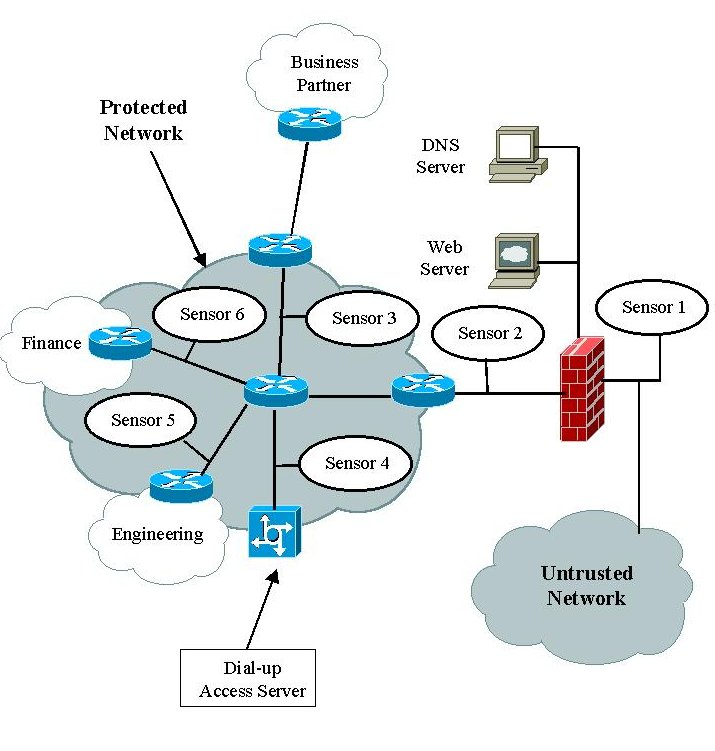
\includegraphics[width=0.95\columnwidth]{images/00/sensores.jpg}
      \caption{Ejemplo de posicionamiento de sensores}
      \label{fig:00/sensores}
   \end{figure}
\end{paracol}

\item \textbf{SIEM (Security Information and Event Management)} \\
Estos sistemas centralizados son fundamentales para la \ul{recopilación, correlación y análisis de eventos} de seguridad procedentes de diferentes fuentes en la red. Los SIEM actúan como el centro neurálgico de las operaciones de seguridad, proporcionando una plataforma unificada donde convergen datos estructurados y no estructurados de múltiples sistemas para crear un contexto coherente. Su capacidad para \ul{normalizar datos heterogéneos} facilita la detección de patrones y anomalías que serían imposibles de percibir examinando cada fuente aisladamente.
\nl

Hemos visto que los SIEM son herramientas potentes, pero \ul{\textit{no} son la solución definitiva} para la CS. Aunque proporcionan una base sólida para la recopilación y análisis de datos, su eficacia depende de la calidad de los datos que reciben y de la capacidad de los analistas para interpretar correctamente los resultados.

\begin{figure}[htbp]
   \centering
   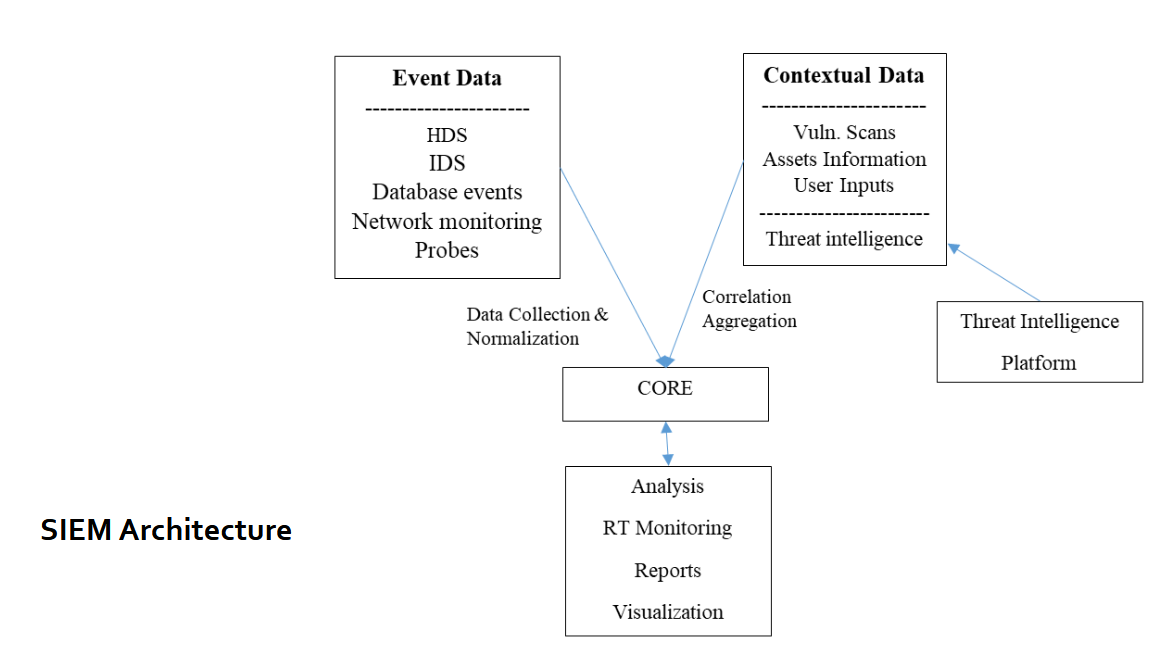
\includegraphics{images/00/SIEM.png}
   \caption{SIEM esquema}
   \label{fig:00/SIEM}
\end{figure}
\end{enumerate}

\section{Dominios físicos y cibernéticos}
\begin{enumerate}[resume]
\item \textbf{Cyber Hybrid Situational Awareness} \\
La integración de la conciencia situacional física y cibernética es esencial porque reconoce que los eventos en un dominio influyen en el otro, proporcionando una visión más completa de las amenazas modernas.\\
Este enfoque híbrido responde a la creciente convergencia entre los mundos físico y digital, donde las fronteras tradicionales se difuminan con la proliferación de \ul{dispositivos IoT}, \ul{sistemas de control industrial} (ICSs) conectados y tecnologías operativas digitalizadas. 
La visión integrada permite detectar amenazas compuestas que utilizan vectores tanto físicos como digitales.

En el caso de los ICS, también es crucial tener en cuenta los \ul{eventos físicos} que pueden influir en la seguridad cibernética, como desastres naturales o fallos de infraestructura, e inversamente, los eventos cibernéticos que pueden tener repercusiones físicas significativas, como la interrupción de servicios críticos o el daño a equipos industriales.\\
Los objetivos de seguridad están en orden inverso de prioridad, siendo la disponibilidad considerada la más importante, en lugar de la confidencialidad.
\note{El personal de la industria a menudo usa el término ``seguridad" para referirse a la disponibilidad y fiabilidad del sistema.
}

\item \textbf{Georreferenciación de activos} \\
La vinculación de activos cibernéticos con elementos físicos es esencial para la situational awareness híbrida, permitiendo visualizar las interdependencias entre el mundo físico y digital. La capacidad de \ul{localizar precisamente los recursos digitales en el espacio físico} proporciona un contexto crucial para interpretar eventos de seguridad, especialmente en organizaciones con presencia geográficamente distribuida o infraestructuras complejas. La georreferenciación permite correlacionar incidentes cibernéticos con eventos físicos próximos.

% \item \textbf{Diferencias entre operaciones cinéticas y cibernéticas} \\
% Comprender las diferencias fundamentales entre ambos dominios es crucial para la CS. Mientras las operaciones cinéticas son \ul{observables físicamente}, dependientes del espacio-tiempo y con efectos lineales inmediatos, las operaciones cibernéticas son \ul{ocultas}, potencialmente sin restricciones espaciales y temporales, y con efectos que pueden manifestarse de forma retardada o no atribuible claramente. Esta distinción fundamental afecta profundamente cómo deben conceptualizarse, monitorizarse y contrarrestarse las amenazas en cada dominio.
\end{enumerate}

\section{Ciberinteligencia para mejorar la CS}
\begin{enumerate}[resume]  % Usa el parámetro resume para continuar la numeración
% \item \textbf{Ciberinteligencia y análisis de amenazas} \\

\item \textbf{Estándares para caracterización e intercambio de información} \\
Los marcos estandarizados como \texttt{STIX}, \texttt{TAXII}, \texttt{OpenIOC} y \texttt{MITRE ATT\&CK} son esenciales para garantizar la interoperabilidad y consistencia en la comunicación de información sobre amenazas entre diferentes organizaciones y herramientas. Estos estándares proporcionan un \ul{lenguaje común} y \ul{estructuras de datos unificadas} que permiten la automatización en el procesamiento e incorporación de inteligencia externa, eliminando la necesidad de conversiones manuales propensas a errores y reduciendo significativamente el tiempo entre la \ul{identificación de una amenaza} y la \ul{implementación de defensas correspondientes}.

\item \textbf{Fuentes de Ciberinteligencia} \\
\begin{figure}[htbp]
   \centering
   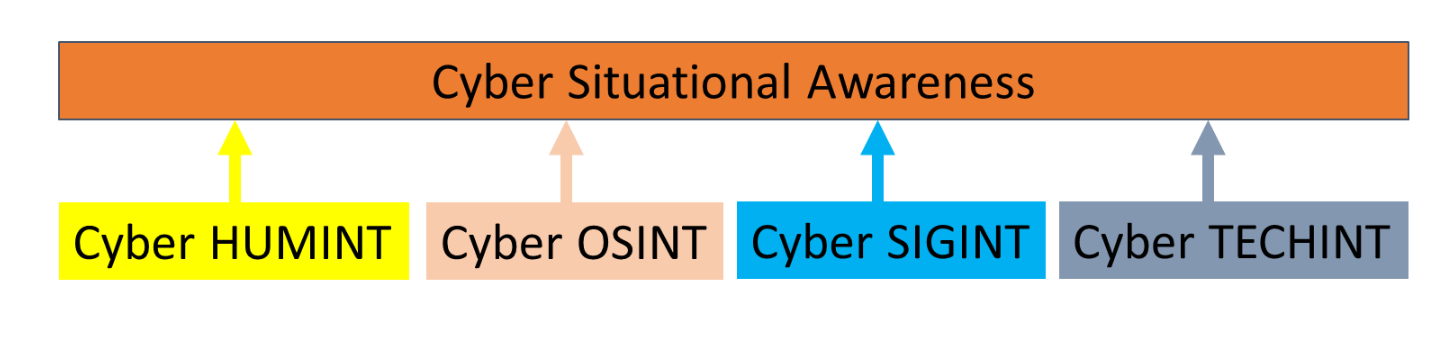
\includegraphics{images/00/CS_CI.png}
   \caption{Ciberinteligencia}
   \label{fig:00/ciberinteligencia}
\end{figure}
La recopilación eficaz de información para la CS se basa en cuatro fuentes distintas y fundamentales de inteligencia.
Esta diversificación de fuentes es crucial porque cada una aporta una perspectiva única y complementaria sobre el panorama de amenazas.
\begin{itemize}
   \item \texttt{HUMINT} - \ul{inteligencia humana}\\
   Proporciona información valiosa sobre intenciones, motivaciones y capacidades de actores maliciosos a través de contactos personales y redes de informantes.
   
   \item \texttt{OSINT} - \ul{inteligencia de fuentes abiertas}\\
   Aprovecha la abundancia de información disponible públicamente para identificar tendencias emergentes, vulnerabilidades recién descubiertas y campañas de ataque en curso. 
   
   \item \texttt{SIGINT} - \ul{inteligencia de señales}\\
   Permite detectar patrones anómalos en las comunicaciones y el tráfico de red que pueden indicar actividades maliciosas. 
   
   \item \texttt{TECHINT} - \ul{inteligencia técnica}\\
   Analiza los artefactos técnicos de ataques (malware, exploits, infraestructura) para comprender las capacidades técnicas de los adversarios y desarrollar contramedidas efectivas.
   
\end{itemize} 


\item \textbf{Sistemas de Respuesta a Incidentes} \\
Los sistemas de respuesta a incidentes son plataformas especializadas que permiten la inserción, almacenamiento y gestión centralizada de incidentes de seguridad, facilitando la coordinación de respuestas efectivas. Son fundamentales porque proporcionan un marco estructurado para el \ul{seguimiento completo del ciclo de vida de los incidentes}, desde su detección inicial hasta su resolución y el análisis posterior. Estos sistemas están diseñados para integrarse con \texttt{TIPs} (Plataformas de Inteligencia de Amenazas) y \texttt{SIEMs}, creando un ecosistema cohesivo de herramientas de seguridad. Ayudan a los miembros del \textit{Computer Incident Response Team} (\texttt{CIRT}) a gestionar adecuadamente los incidentes, proporcionando gestión de flujos de trabajo y registros detallados sobre qué ocurrió, cuándo y cómo, tanto respecto al incidente como a la respuesta implementada. La documentación meticulosa que facilitan estos sistemas es invaluable para el aprendizaje organizacional, permitiendo refinar continuamente los procedimientos de respuesta basándose en experiencias previas y adaptarse a tácticas de ataque en evolución.

% \item \textbf{Gráficos de escenarios de ataque} \\
% Los \textit{attack scenario graphs} son una herramienta avanzada de visualización que representa las relaciones entre las vulnerabilidades de un sistema y muestra cómo pueden desarrollarse ataques multi-etapa. Son fundamentales para la CS porque permiten anticipar posibles rutas de compromiso antes de que sean explotadas por atacantes. Estos gráficos pueden vincularse con \texttt{software dependency graphs} para visualizar cómo un paso de ataque a un componente puede afectar a otros componentes dependientes, creando un modelo completo de la superficie de ataque. La representación visual de estas relaciones facilita la identificación de puntos críticos donde una sola vulnerabilidad podría desencadenar efectos en cascada a través de múltiples sistemas. Esta perspectiva estructurada supera las limitaciones de los enfoques tradicionales que solo consideran vulnerabilidades individuales, permitiendo priorizar defensas basadas no solo en la gravedad de vulnerabilidades aisladas, sino también en su posición estratégica dentro de posibles cadenas de ataque.

% \newpage

\item \textbf{Attack Graphs}\\
Los \textit{attack graphs} son representaciones gráficas que ilustran las relaciones entre vulnerabilidades y cómo pueden ser explotadas en una secuencia de pasos para comprometer un sistema. Son fundamentales para la CS porque permiten \ul{visualizar la complejidad de los ataques} y sus \ul{posibles consecuencias en cascada}, facilitando la identificación de puntos críticos. Estos gráficos ayudan a los analistas a comprender cómo un atacante podría navegar a través de un entorno, aprovechando múltiples vulnerabilidades interconectadas para lograr su objetivo.

\begin{figure}[htbp]
   \centering
   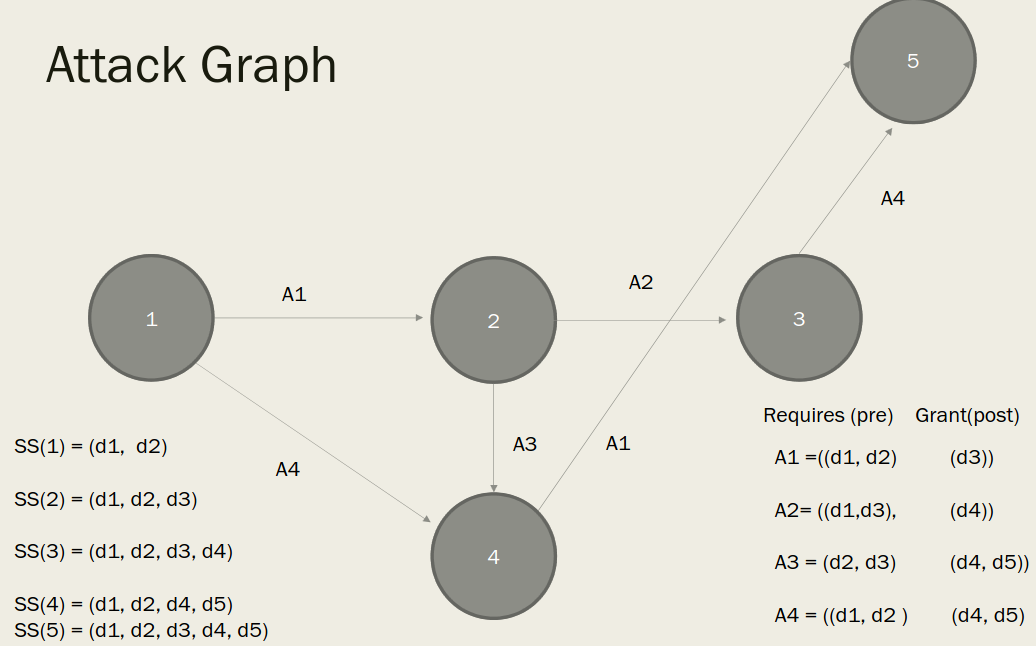
\includegraphics[width=0.45\columnwidth]{images/00/attackgraph.png}
   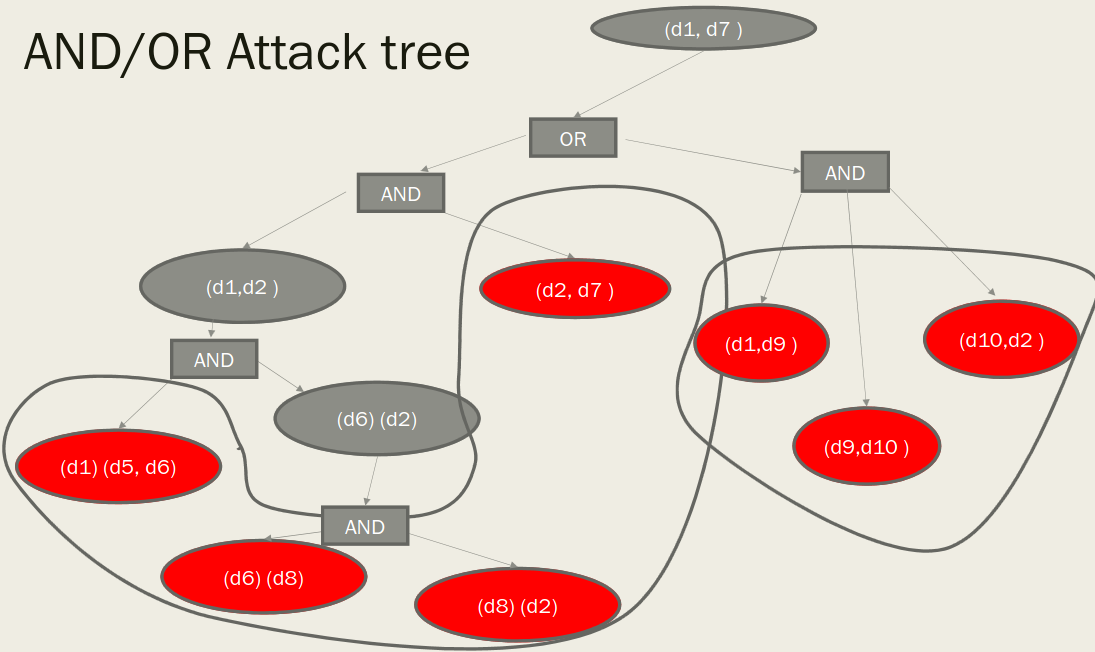
\includegraphics[width=0.45\columnwidth]{images/00/attacktree.png}
   \label{fig:00/attackgraph}
   \caption{Ejemplo de un attack graph y de un attack tree}
   $SS$ es el Security Status, los derechos de acceso ($d1,d2,d3,\dots$) obtenidos por el atacante mediante ataques anteriores.
   \nl

   {En el attack \textit{tree}:\ns
      \begin{itemize}
         \item Una hoja representa un ataque permitido por una vulnerabilidad = un ataque elemental
         \item Un nodo que no es una hoja representa un ataque complejo
         \item El subtree enraizado en el nodo muestra cómo puede implementarse un ataque complejo
      \end{itemize}}
\end{figure}

Esta representación visual no solo mejora la comprensión de las amenazas, sino que también permite priorizar defensas y mitigaciones basadas en la probabilidad de explotación de diferentes rutas de ataque.\\
Es posible detener una intrusión calculando cortes en un grafo de ataque.
\begin{figure}[htbp]
   \centering
   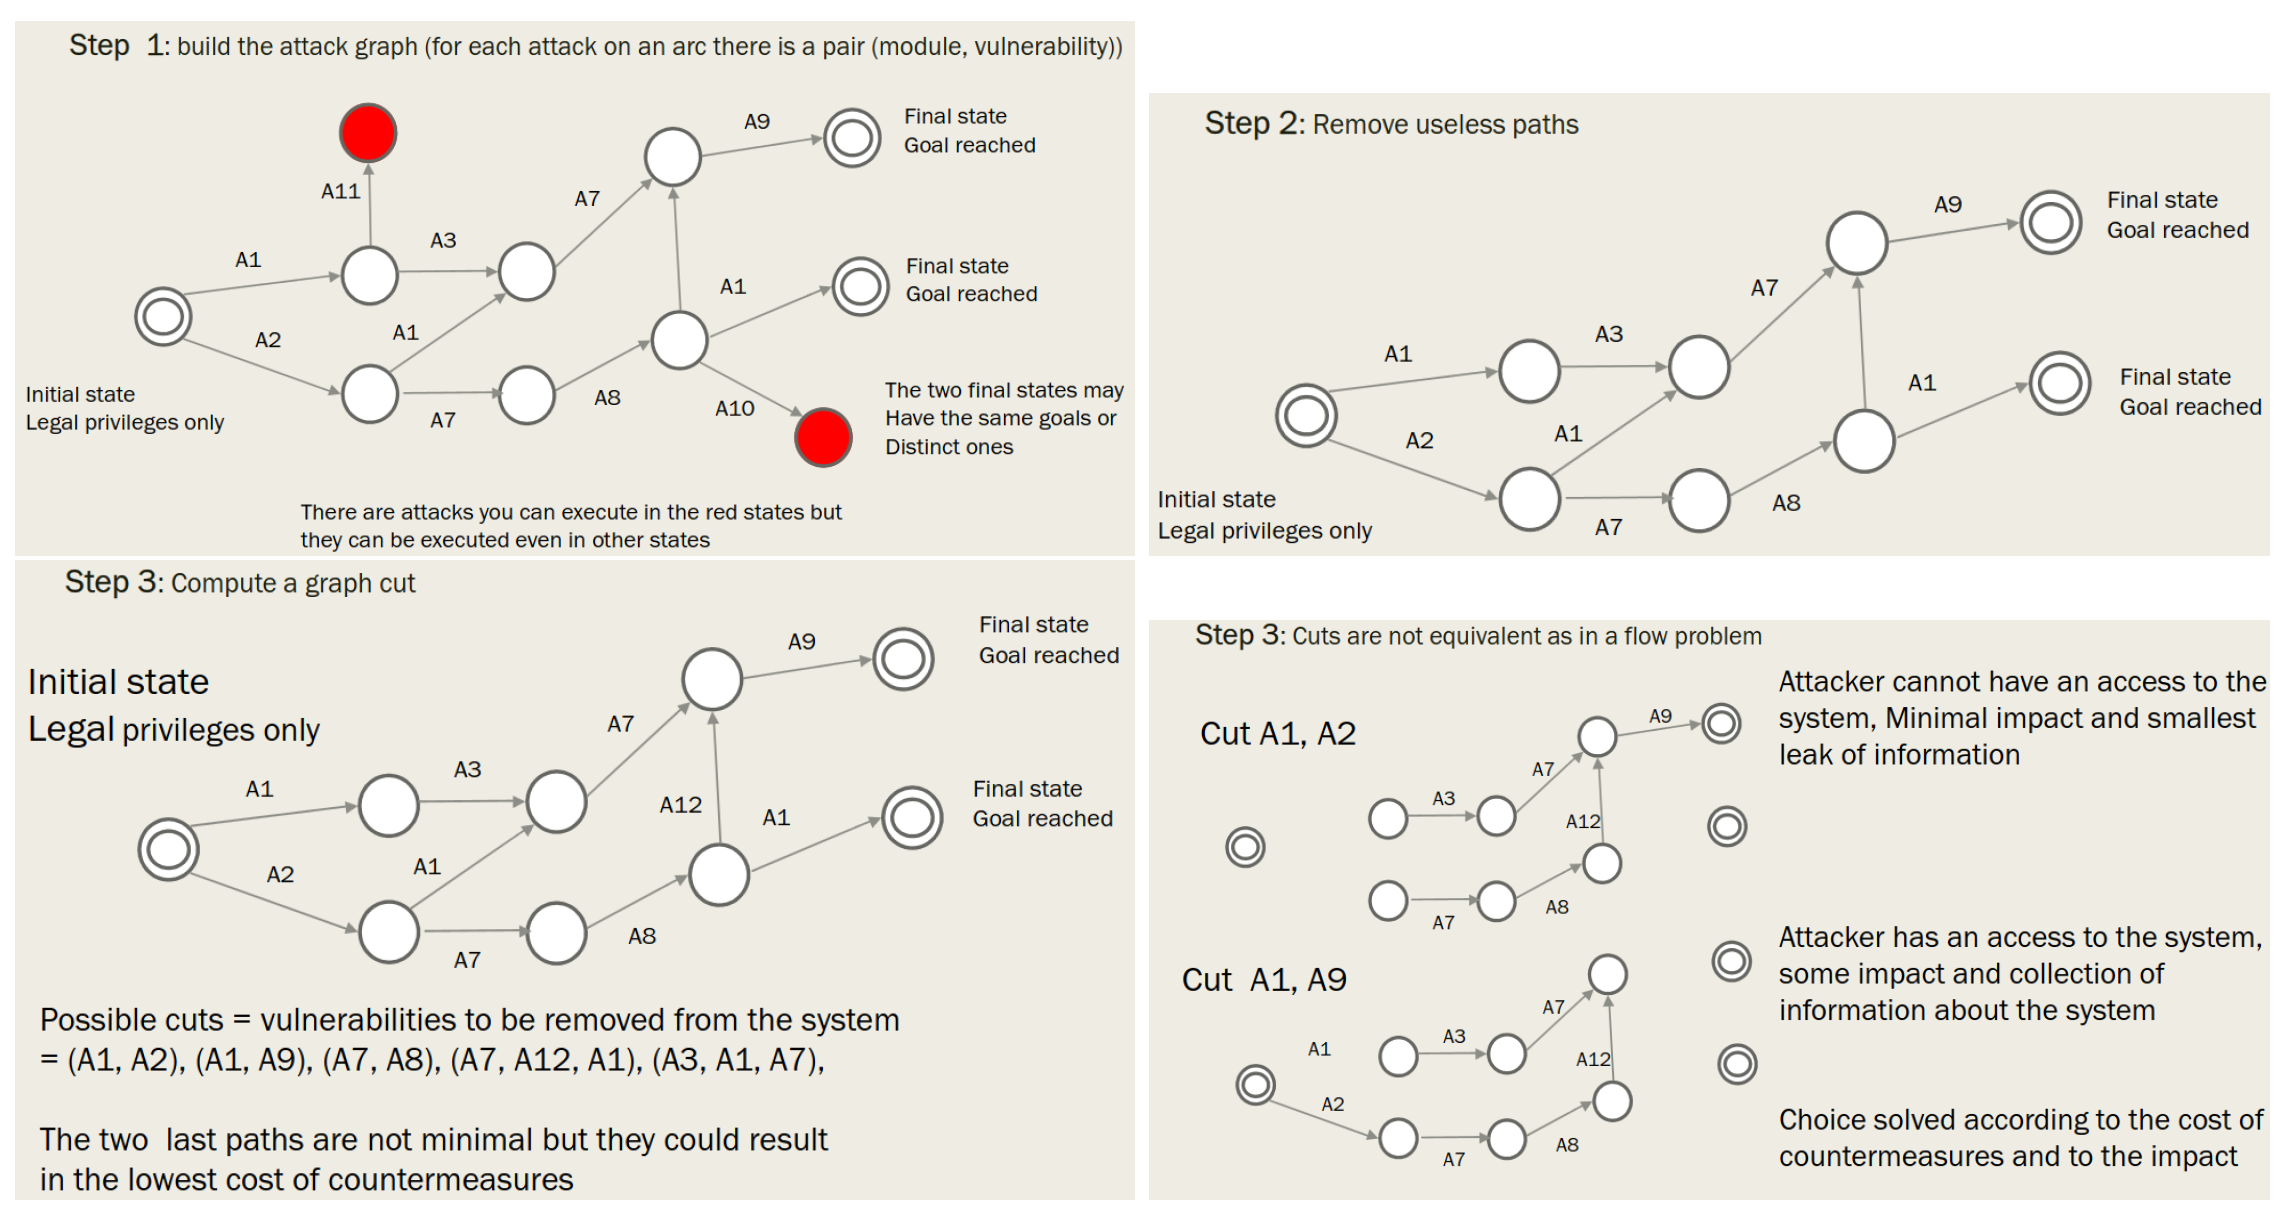
\includegraphics{images/00/graphintrusions.png}
   \caption{Detener una intrusión calculando cortes en un grafo de ataque}
   \label{fig:00/graphintrusions}
\end{figure}

\item \textbf{Niveles de mando CS: Táctico, Operativo y Estratégico} \\
La subdivisión de la conciencia situacional en los niveles táctico, operativo y estratégico es crucial porque permite adaptar la información a las necesidades específicas de los diferentes niveles decisionales. 
\begin{itemize}
   \item El nivel \textbf{táctico} (a veces llamado \textit{técnico}) se enfoca en visualizar y gestionar eventos relacionados con activos específicos, requiriendo información detallada y técnica para la detección y respuesta inmediata a incidentes
   \item El nivel \textbf{operativo} busca sintetizar los detalles del nivel táctico y contextualizarlos en términos de su impacto en la misión organizacional, facilitando la coordinación de múltiples acciones tácticas dentro de un marco temporal más amplio
   \item El nivel \textbf{estratégico} requiere información abstracta y contextualizada sobre el panorama general de amenazas y su posible impacto en los objetivos organizacionales a largo plazo, permitiendo la planificación defensiva, la asignación de recursos y el alineamiento con requisitos regulatorios. Esta estructura jerárquica asegura que cada nivel reciba la información con el grado apropiado de detalle y abstracción.
\end{itemize}

Esta division es importante se encuentra más comunemente en el contexto militar, pero su aplicacion es igualmente relevante en el ámbito de la ciberseguridad, y permite de haber un ``framework''/enfoque común para la CS.
\end{enumerate}